\documentclass{beamer}

\pdfmapfile{+sansmathaccent.map}


\mode<presentation>
{
	\usetheme{Warsaw} % or try Darmstadt, Madrid, Warsaw, Rochester, CambridgeUS, ...
	\usecolortheme{seahorse} % or try seahorse, beaver, crane, wolverine, ...
	\usefonttheme{serif}  % or try serif, structurebold, ...
	\setbeamertemplate{navigation symbols}{}
	\setbeamertemplate{caption}[numbered]
} 


%%%%%%%%%%%%%%%%%%%%%%%%%%%%
% itemize settings

\definecolor{myhotpink}{RGB}{255, 80, 200}
\definecolor{mywarmpink}{RGB}{255, 60, 160}
\definecolor{mylightpink}{RGB}{255, 80, 200}
\definecolor{mypink}{RGB}{255, 30, 80}
\definecolor{mydarkpink}{RGB}{155, 25, 60}

\definecolor{mypaleblue}{RGB}{240, 240, 255}
\definecolor{mylightblue}{RGB}{120, 150, 255}
\definecolor{myblue}{RGB}{90, 90, 255}
\definecolor{mygblue}{RGB}{70, 110, 240}
\definecolor{mydarkblue}{RGB}{0, 0, 180}
\definecolor{myblackblue}{RGB}{40, 40, 120}

\definecolor{mygreen}{RGB}{0, 200, 0}
\definecolor{mygreen2}{RGB}{245, 255, 230}

\definecolor{mygray}{gray}{0.8}
\definecolor{mydarkgray}{RGB}{80, 80, 160}

\definecolor{mydarkred}{RGB}{160, 30, 30}
\definecolor{mylightred}{RGB}{255, 150, 150}
\definecolor{myred}{RGB}{200, 110, 110}
\definecolor{myblackred}{RGB}{120, 40, 40}

\definecolor{mygreen}{RGB}{0, 200, 0}
\definecolor{mygreen2}{RGB}{205, 255, 200}

\definecolor{mydarkcolor}{RGB}{60, 25, 155}
\definecolor{mylightcolor}{RGB}{130, 180, 250}

\setbeamertemplate{itemize items}[default]

\setbeamertemplate{itemize item}{\color{myblackblue}$\blacksquare$}
\setbeamertemplate{itemize subitem}{\color{mydarkblue}$\blacktriangleright$}
\setbeamertemplate{itemize subsubitem}{\color{mygray}$\blacksquare$}

\setbeamercolor{palette quaternary}{fg=white,bg=mygblue} %mydarkgray
\setbeamercolor{titlelike}{parent=palette quaternary}

\setbeamercolor{palette quaternary2}{fg=white,bg=mygblue}%black myblue
\setbeamercolor{frametitle}{parent=palette quaternary2}

\setbeamerfont{frametitle}{size=\Large,series=\scshape}
\setbeamerfont{framesubtitle}{size=\normalsize,series=\upshape}


%%%%%%%%%%%%%%%%%%%%%%%%%%%%
% block settings

%\setbeamercolor{block title}{bg=red!50,fg=black}
%\setbeamercolor{block title}{bg=mylightblue,fg=black}
\setbeamercolor{block title}{bg=myblackblue,fg=white}

\setbeamercolor*{block title example}{bg=mygreen!40!white,fg=black}

\setbeamercolor*{block body example}{fg= black,
	bg= mygreen2}


%%%%%%%%%%%%%%%%%%%%%%%%%%%%
% URL settings
\hypersetup{
	colorlinks=false,
	linkcolor=blue,
	filecolor=blue,      
	urlcolor=blue,
}

%%%%%%%%%%%%%%%%%%%%%%%%%%

\renewcommand{\familydefault}{\rmdefault}

\usepackage{amsmath}
\usepackage{mathtools}

\usepackage{subcaption}

\usepackage{qrcode}

\DeclareMathOperator*{\argmin}{arg\,min}
\newcommand{\bo}[1] {\mathbf{#1}}

\newcommand{\dx}[1] {\dot{\mathbf{#1}}}
\newcommand{\ma}[4] {\begin{bmatrix}
		#1 & #2 \\ #3 & #4
\end{bmatrix}}
\newcommand{\myvec}[2] {\begin{bmatrix}
		#1 \\ #2
\end{bmatrix}}
\newcommand{\myvecT}[2] {\begin{bmatrix}
		#1 & #2
\end{bmatrix}}

\newcommand{\R}{\mathbb{R}} 
\newcommand{\T}{^\top}     



\newcommand{\mydate}{Spring 2023}

\newcommand{\mygit}{\textcolor{blue}{\href{https://github.com/SergeiSa/Computational-Intelligence-Slides-Spring-2023}{github.com/SergeiSa/Computational-Intelligence-Slides-Spring-2023}}}

\newcommand{\myqr}{ \textcolor{black}{\qrcode[height=1.5in]{https://github.com/SergeiSa/Computational-Intelligence-Slides-Spring-2023}}
}

\newcommand{\myqrframe}{
	\begin{frame}
		\centerline{Lecture slides are available via Github, links are on Moodle}
		\bigskip
		\centerline{You can help improve these slides at:}
		\centerline{\mygit}
		\bigskip
		\myqr
	\end{frame}
}


\newcommand{\bref}[2] {\textcolor{blue}{\href{#1}{#2}}}



%%%%%%%%%%%%%%%%%%%%%%%%%%%%
% code settings

\usepackage{listings}
\usepackage{color}
% \definecolor{mygreen}{rgb}{0,0.6,0}
% \definecolor{mygray}{rgb}{0.5,0.5,0.5}
\definecolor{mymauve}{rgb}{0.58,0,0.82}
\lstset{ 
	backgroundcolor=\color{white},   % choose the background color; you must add \usepackage{color} or \usepackage{xcolor}; should come as last argument
	basicstyle=\footnotesize,        % the size of the fonts that are used for the code
	breakatwhitespace=false,         % sets if automatic breaks should only happen at whitespace
	breaklines=true,                 % sets automatic line breaking
	captionpos=b,                    % sets the caption-position to bottom
	commentstyle=\color{mygreen},    % comment style
	deletekeywords={...},            % if you want to delete keywords from the given language
	escapeinside={\%*}{*)},          % if you want to add LaTeX within your code
	extendedchars=true,              % lets you use non-ASCII characters; for 8-bits encodings only, does not work with UTF-8
	firstnumber=0000,                % start line enumeration with line 0000
	frame=single,	                   % adds a frame around the code
	keepspaces=true,                 % keeps spaces in text, useful for keeping indentation of code (possibly needs columns=flexible)
	keywordstyle=\color{blue},       % keyword style
	language=Octave,                 % the language of the code
	morekeywords={*,...},            % if you want to add more keywords to the set
	numbers=left,                    % where to put the line-numbers; possible values are (none, left, right)
	numbersep=5pt,                   % how far the line-numbers are from the code
	numberstyle=\tiny\color{mygray}, % the style that is used for the line-numbers
	rulecolor=\color{black},         % if not set, the frame-color may be changed on line-breaks within not-black text (e.g. comments (green here))
	showspaces=false,                % show spaces everywhere adding particular underscores; it overrides 'showstringspaces'
	showstringspaces=false,          % underline spaces within strings only
	showtabs=false,                  % show tabs within strings adding particular underscores
	stepnumber=2,                    % the step between two line-numbers. If it's 1, each line will be numbered
	stringstyle=\color{mymauve},     % string literal style
	tabsize=2,	                   % sets default tabsize to 2 spaces
	title=\lstname                   % show the filename of files included with \lstinputlisting; also try caption instead of title
}

%%%%%%%%%%%%%%%%%%%%%%%%%%%%
% tikz settings

\usepackage{tikz}
\tikzset{every picture/.style={line width=0.75pt}}

%%%%%%%%%%%%%%%%%%%%%%%%%%%%




\title{Least Squares and Quadratic Programming}
\subtitle{Computational Intelligence, Lecture 3}
\author{by Sergei Savin}
\centering
\date{\mydate}



\begin{document}
\maketitle


%\begin{frame}{Content}
%
%\begin{itemize}
%\item Problems with analytical solutions
%\item Problems with inequality constraints
%\item Quadratic programming
%\item Homework
%\end{itemize}
%
%\end{frame}



\begin{frame}{Problems with analytical solutions}
% \framesubtitle{Parameter estimation}
\begin{flushleft}

Problem 1. $\text{minimize} \ ||\mathbf{x}||$. Solution $\mathbf{x} = \mathbf{0}$.

\bigskip

Problem 2. $\text{minimize} \ ||\mathbf{A}\mathbf{x}||$. Solution $\mathbf{x} = \mathbf{0}$.

\bigskip

Problem 3. $\text{minimize} \ ||\mathbf{A}\mathbf{x} + \mathbf{b}||$. 

\bigskip

We know solution of $\text{minimize} \ ||\mathbf{A}\mathbf{x} - \mathbf{b}||$, which is $\mathbf{x} = \mathbf{A}^+ \mathbf{b}$. Therefore the problem 3 has a solution $\mathbf{x} = -\mathbf{A}^+ \mathbf{b}$.
 
\end{flushleft}
\end{frame}




\begin{frame}{Problems with analytical solutions}
%\framesubtitle{Part 3}
\begin{flushleft}


Problem 4. 
%
\begin{equation}
\begin{aligned}
& \underset{\mathbf{x}}{\text{minimize}}
& & || \mathbf{x} ||, \\
& \text{subject to}
& & \mathbf{A} \mathbf{x} = \mathbf{c}.
\end{aligned}
\end{equation}


All solutions to $\mathbf{A} \mathbf{x} = \mathbf{c}$ are written as $\mathbf{x} = \mathbf{A}^+\mathbf{c} + \mathbf{N}\mathbf{z}$, where $\mathbf{N} = \text{null}(\mathbf{A})$, and $\mathbf{A}^+\mathbf{c} \in \text{row}(\mathbf{A})$ as we proved previously. Since null space solution $\mathbf{N}\mathbf{z}$ and row space paricular solution $\mathbf{A}^+\mathbf{c}$ are orthagonal, the minimum norm solution corresponds to $\mathbf{z} = \mathbf{0}$, hence $\mathbf{x} = \mathbf{A}^+\mathbf{c}$.



\end{flushleft}
\end{frame}



\begin{frame}{Problems with analytical solutions}
%\framesubtitle{Part 4}
\begin{flushleft}


Thus, the solution is  $\mathbf{x} = \mathbf{A}^+\mathbf{c}$. Notice that solutions for the problem 4 and problem 3 are written identically (sans the sign), even though problem 3 asks us to minimize residual of the linear system, while problem 4 - find minimum norm solution. 

\bigskip

This illustrates an important fact that solution to the least squares problem, formulated either as "minimization of a residual" or as a "minimum norm solution" are given by the same formula, which we call Moore-Penrose pseudoinverse.


\end{flushleft}
\end{frame}





\begin{frame}{Problems with analytical solutions}
%\framesubtitle{Part 4}
\begin{flushleft}

Problem 5. 
%
\begin{equation}
\begin{aligned}
& \underset{\mathbf{x}}{\text{minimize}}
& & || \mathbf{D}\mathbf{x} ||, \\
& \text{subject to}
& & \mathbf{A} \mathbf{x} = \mathbf{b}.
\end{aligned}
\end{equation}

One way to think about it is to first find all solution to the constraint equation $\mathbf{A} \mathbf{x} = \mathbf{b}$ and then find optimal one among them. As we know, all solutions are given as: $\mathbf{x} = \mathbf{A}^+\mathbf{b} + \mathbf{N}\mathbf{z}$, where $\mathbf{N} = \text{null}(\mathbf{A})$. Then our cost function becomes: $|| \mathbf{D}\mathbf{A}^+\mathbf{b} +  \mathbf{D}\mathbf{N}\mathbf{z} ||$, which is equivalent to the problem 3. Thus, we can write solution as: 
$\mathbf{z}^* = -(\mathbf{D}\mathbf{N})^+ \mathbf{D}\mathbf{A}^+\mathbf{b}$. In terms of $\mathbf{x}$ solution is:

\begin{equation}
    \mathbf{x}^* = \mathbf{A}^+\mathbf{b}-\mathbf{N}(\mathbf{D}\mathbf{N})^+ \mathbf{D}\mathbf{A}^+\mathbf{b}
\end{equation}
\begin{equation}
	\mathbf{x}^* =( \mathbf{I}-\mathbf{N}(\mathbf{D}\mathbf{N})^+ \mathbf{D})\mathbf{A}^+\mathbf{b}
\end{equation}

\end{flushleft}
\end{frame}



\begin{frame}{Problems with analytical solutions}
%\framesubtitle{Part 5}
\begin{flushleft}

Problem 6. 
%
\begin{equation}
\begin{aligned}
& \underset{\mathbf{x}}{\text{minimize}}
& & || \mathbf{D}\mathbf{x} + \mathbf{f} ||, \\
& \text{subject to}
& & \mathbf{A} \mathbf{x} = \mathbf{b}.
\end{aligned}
\end{equation}

After the same initial step, we arrive at the cost function $|| \mathbf{D}\mathbf{N}\mathbf{z} + \mathbf{D}\mathbf{A}^+\mathbf{b} + \mathbf{f}||$. It is only different in the constant term, and the solution is found as follows:


\begin{equation}
    \mathbf{z}^* = -(\mathbf{D}\mathbf{N})^+ (\mathbf{D}\mathbf{A}^+\mathbf{b} + \mathbf{f})
\end{equation}
\begin{equation}
    \mathbf{x}^* = \mathbf{A}^+\mathbf{b}-\mathbf{N}(\mathbf{D}\mathbf{N})^+ (\mathbf{D}\mathbf{A}^+\mathbf{b} + \mathbf{f})
\end{equation}


\end{flushleft}
\end{frame}



\begin{frame}{Problems with analytical solutions}
%\framesubtitle{Part 6}
\begin{flushleft}

Problem 7. 
%
\begin{equation}
\begin{aligned}
& \underset{\mathbf{x}}{\text{minimize}}
& & \mathbf{x}^\top \mathbf{H} \mathbf{x} + \mathbf{c}^\top\mathbf{x}, \\
& \text{subject to}
& & \mathbf{A} \mathbf{x} = \mathbf{b}.
\end{aligned}
\end{equation}

where $\mathbf{H}$ is positive-definite.

\bigskip

Assume that we found a decomposition $\mathbf{H} = \mathbf{D}^\top\mathbf{D}$. We can also find such $\mathbf{f}$ that $2\mathbf{f}^\top\mathbf{D} = \mathbf{c}^\top$. Then our cost function becomes $\mathbf{x}^\top \mathbf{D}^\top\mathbf{D} \mathbf{x} + 2\mathbf{f}^\top\mathbf{D}\mathbf{x}$, which as we saw before has coinciding minimum with the cost function $||\mathbf{D}\mathbf{x} + \mathbf{f}||$.

\bigskip

Therefore the problem has the same solution as Problem 5, after the mentioned above change in constants.

\end{flushleft}
\end{frame}




\begin{frame}{Problems with inequality constraints}
% \framesubtitle{Part 1}
\begin{flushleft}

Problem 9. 
%
\begin{equation}
\begin{aligned}
& \underset{\mathbf{x}}{\text{minimize}}
& & || \mathbf{D}\mathbf{x} + \mathbf{f} ||, \\
& \text{subject to}
& & \mathbf{x} \leq \mathbf{b}.
\end{aligned}
\end{equation}

Problem 10. 
%
\begin{equation}
\begin{aligned}
& \underset{\mathbf{x}}{\text{minimize}}
& & || \mathbf{x} ||, \\
& \text{subject to}
& & \mathbf{A}\mathbf{x} \leq \mathbf{b}.
\end{aligned}
\end{equation}

Problem 11. 
%
\begin{equation}
\begin{aligned}
& \underset{\mathbf{x}}{\text{minimize}}
& & || \mathbf{D}\mathbf{x} + \mathbf{f} ||, \\
& \text{subject to}
& & \begin{cases}
    \mathbf{A}\mathbf{x} \leq \mathbf{b}, \\
    \mathbf{C}\mathbf{x} = \mathbf{d}.
    \end{cases}
\end{aligned}
\end{equation}

\end{flushleft}
\end{frame}



\begin{frame}{Quadratic programming}
% \framesubtitle{Part 1}
\begin{flushleft}

Mentioned problems can be described together as quadratic programs. The name is due to the cost function being quadratic (or equivalent). They are allowed to have linear equality or inequality constraints. 

\bigskip

General form of a quadratic program is given below:

%
\begin{equation}
\begin{aligned}
& \underset{\mathbf{x}}{\text{minimize}}
& & \mathbf{x}^\top \mathbf{H} \mathbf{x} + \mathbf{f}^\top\mathbf{x}, \\
& \text{subject to}
& & \begin{cases}
    \mathbf{A}\mathbf{x} \leq \mathbf{b}, \\
    \mathbf{C}\mathbf{x} = \mathbf{d}.
    \end{cases}
\end{aligned}
\end{equation}

where $\mathbf{H}$ is positive-definite and $\mathbf{A}\mathbf{x} \leq \mathbf{b}$ describe a \emph{convex region}.

\end{flushleft}
\end{frame}




\begin{frame}{Domain}
	% \framesubtitle{Parameter estimation}
	\begin{flushleft}
		
		\centerline{Domain, Convexity}
		
	\end{flushleft}
\end{frame}



\begin{frame}{Domain}
	% \framesubtitle{Parameter estimation}
	\begin{flushleft}
		
		Problem 1. Find minimum of the function $f = x^2 + 2y^2$ if $x \in \mathbb{R}$ and $y \in \mathbb{R}$. Solution is $x = 0$, $y = 0$.
		
		\bigskip
		
		Problem 2. Find minimum of the function $f = x^2 + 2y^2$ if $x \in [1 \ 2]$ and $y \in [2 \ 5]$. Solution is $x = 1$, $y = 2$.
		
		\bigskip
		
		Note that solutions of problems 1 and 2 are different, and this is only due to the difference of the allowed values that the \emph{decision variables} $x$ and $y$ can assume.
		
		\begin{block}{Definition 1}
			Space of all allowed values that decision variables can assume is called the \emph{domain} of optimization problem.
		\end{block}
		
	\end{flushleft}
\end{frame}



\begin{frame}{Bounded and unbounded domains}
	\framesubtitle{Part 1}
	\begin{flushleft}
		
		Problem 3. Find minimum of the function $f = -x^2$ if $x \in [-3 \ 2]$. Solution is $x = -3$.
		
		\bigskip
		
		Problem 4. Find minimum of the function $f = -x^2$ if $x \in \mathbb{R}$. The problem has no solution.
		
		\bigskip
		
		Problem 5. Find minimum of the function $f = -x^2$ if $x \in  [-\infty \ 2]$. The problem has no solution.
		
		\bigskip
		
		The major difference between domains of the problems 2, 3 vs problems 1, 4 and 5 is that the later are \emph{not bound} (i.e., you can construct a sequence of the values in the domain that would approach infinity).
		
		\bigskip
		
		We can see that in the case of problems 3-5, bounded domain allows the problem to have a solution.
		
	\end{flushleft}
\end{frame}



\begin{frame}{Bounded and unbounded domains}
	\framesubtitle{Part 2}
	\begin{flushleft}
		
		Problem 6. Find maximum of the function $f = x^2$ if $1 \leq x < 2$. It has no solution.
		
		\bigskip
		
		Problem 7. Find minimum of the function $f = x^2$ if $1 \leq x < 2$. Solution is $x = 1$.
		
		\bigskip
		
		This time, it is the fact that one of the \emph{boundaries} of the domain was not included in the domain that has lead the problem 6 to have no solution, while problem 7 had one. For the problem 6 we can pick a value arbitrary close to $x = 2$, approaching it from the left, but for any such value, there always will be other values of the decision variable closer to $x = 2$ and hence producing larger values of $f$.
		
	\end{flushleft}
\end{frame}


\begin{frame}{Convex domains}
	% \framesubtitle{Parameter estimation}
	\begin{flushleft}
		
		\begin{block}{Definition 2}
			Domain is \emph{convex} iff for any two points in the domain, the line segment connecting them is also in the domain.
		\end{block}
		
		\bigskip
		
		\begin{figure}
			\centering
			\begin{minipage}{.3\textwidth}
				\centering
				
				\textit{  
					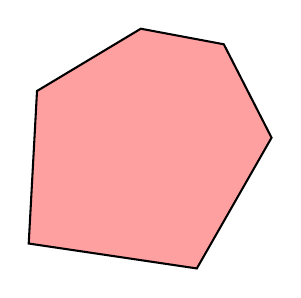
\begin{tikzpicture}[x=0.75pt,y=0.75pt,yscale=-1,xscale=1]
						\draw  [fill={rgb, 255:red, 255; green, 160; blue, 160 }  ,fill opacity=1 ] (148,55) -- (188,62.5) -- (211,107.5) -- (175,170.5) -- (94,158.5) -- (98,85) -- cycle ;
				\end{tikzpicture}}
				
				\captionof{figure}{Convex domain}
			\end{minipage}%
			\begin{minipage}{.7\textwidth}
				\centering
				
				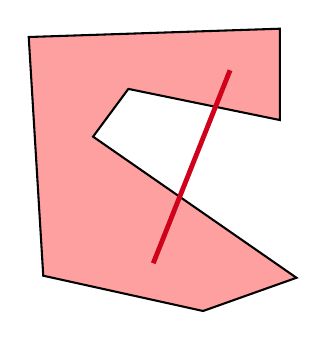
\begin{tikzpicture}[x=0.75pt,y=0.75pt,yscale=-1,xscale=1]
					\draw  [fill={rgb, 255:red, 255; green, 160; blue, 160 }  ,fill opacity=1 ] (525,68.5) -- (525,112.5) -- (452,97.5) -- (435,120.5) -- (533,188.5) -- (488,204.5) -- (411,187.5) -- (404,72.5) -- cycle ;
					\draw [color={rgb, 255:red, 208; green, 2; blue, 27 }  ,draw opacity=1, line width=1.75pt ]   (501,88.5) -- (486.03,126.12) -- (464,181.5) ;
				\end{tikzpicture}
				
				\captionof{figure}{Non-convex domain}
			\end{minipage}
		\end{figure}
		
	\end{flushleft}
\end{frame}





\begin{frame}{Convex combination}
	% \framesubtitle{Parameter estimation}
	\begin{flushleft}
		
		
		In the proofs it is convenient to remember that for any two points $\mathbf{x}_1$ and $\mathbf{x}_2$, all points in the line segment connecting them are given as $\mathbf{x}_l = \alpha \mathbf{x}_1 + (1 - \alpha) \mathbf{x}_2$, where $\alpha \in [0 \ 1]$. This is called \emph{convex combination}.
		
		
	\end{flushleft}
\end{frame}



\begin{frame}{Examples of convex domains}
	% \framesubtitle{Parameter estimation}
	\begin{flushleft}
		
		$\mathbf{x} \in \mathcal{X}$, $\mathcal{X} = \mathbb{R}^n$  is convex.
		
		\bigskip
		
		$\mathbf{x} \in \mathcal{X}$, $\mathcal{X} = \{ \mathbf{x} \in \mathbb{R}^n: \ \mathbf{x} \leq \mathbf{h} \}$ is convex.
		
		\bigskip
		
		Proof: Note that $\alpha \mathbf{x}_1 \leq \alpha \mathbf{h}$ and $(1 - \alpha) \mathbf{x}_2 \leq (1 - \alpha) \mathbf{h}$, hence, $\alpha \mathbf{x}_1 + (1 - \alpha) \mathbf{x}_2 \leq 
		\alpha \mathbf{h} + (1 - \alpha) \mathbf{h} = \mathbf{h}$. \qedsymbol
		
		\bigskip
		
		$\mathbf{x} \in \mathcal{X}$, $\mathcal{X} = \{ \mathbf{x} \in \mathbb{R}^2: \ x_1^2+x_2^2 \leq h^2 \}$ is convex.
		
		\bigskip
		
		Proof: This is the same as $|| \mathbf{x} || \leq h$. Note that $|| \alpha \mathbf{x}_1 || \leq \alpha h$ and $|| (1 - \alpha) \mathbf{x}_2 || \leq (1 - \alpha) h$, also 
		
		$$|| \alpha \mathbf{x}_1 + (1 - \alpha) \mathbf{x}_2 || \leq || \alpha \mathbf{x}_1 || + || (1 - \alpha) \mathbf{x}_2 ||$$
		$$|| \alpha \mathbf{x}_1 || + || (1 - \alpha) \mathbf{x}_2 || \leq \alpha h + (1 - \alpha) h = h$$ 
		
		So the convex combination of $\mathbf{x}_1$ and $\mathbf{x}_2$ is still in the domain. \qedsymbol
		
		
	\end{flushleft}
\end{frame}






\begin{frame}{Examples of convex domains}
	% \framesubtitle{Parameter estimation}
	\begin{flushleft}
		
		$\mathbf{x} \in \mathcal{X}$, $\mathcal{X} = \{ \mathbf{x} \in \mathbb{R}^n: \ \mathbf{x}^\top \mathbf{H} \mathbf{x} \leq 1 \}$, where $\mathbf{H} \succ 0$ is positive-definite symmetric matrix is convex. 
		
		\bigskip
		
		For any positive-definite symmetric $\mathbf{H}$ it is true that $\mathbf{H} = \mathbf{D}^\top\mathbf{D}$, where $\mathbf{D} = \sqrt{\mathbf{H}}$ is called a matrix square root and it is full rank. With that $\mathbf{x}^\top \mathbf{H} \mathbf{x} \leq 1$ becomes $\mathbf{x}^\top \mathbf{D}^\top\mathbf{D} \mathbf{x} \leq 1$. Defining $\mathbf{y} = \mathbf{D} \mathbf{x}$ we get $\mathcal{X} = \{ \mathbf{D}^{-1}\mathbf{y}: \ \mathbf{y}^\top \mathbf{y} \leq 1 \}$. This is a linearly deformed previously covered domain, and as such it is also convex.
		
	\end{flushleft}
\end{frame}



\begin{frame}{Examples of non-convex domains}
	% \framesubtitle{Parameter estimation}
	\begin{flushleft}
		
		%$\mathbf{x} \in \mathcal{X}$, $\mathcal{X} = \{ \mathbf{x} \in \mathbb{R}^n: \ \mathbf{x} \geq \mathbf{h} \}$ is not convex. Prove it.
		%
		%\bigskip
		
		$x \in \mathcal{X}$, $\mathcal{X} = [-1 \ 2] \cup [3 \ 7]$ is not convex..
		
		\bigskip
		
		$\mathbf{x} \in \mathcal{X}$, $\mathcal{X} = \{ \mathbf{x} \in \mathbb{R}^2: \ x_1^2+x_2^2 \geq h^2 \}$ is not convex. Prove it.
		
		\bigskip
		
		$\mathbf{x} \in \mathcal{X}$, $\mathcal{X} = \{ \mathbf{x} \in \mathbb{R}^n: \ \mathbf{x}^\top \mathbf{H} \mathbf{x} \geq 1 \}$, where $\mathbf{H}$ is positive-definite symmetric matrix is not convex. Prove it.
		
		\bigskip
		
		These proves simply require one counter-example to show that the defining property of convex domains does not hold.
		
	\end{flushleft}
\end{frame}




\begin{frame}{Convex functions}
	% \framesubtitle{Parameter estimation}
	\begin{flushleft}
		
		\begin{block}{Definition 3}
			Function $f(\mathbf{x})$ defined on a domain $\mathcal{D}$, for which it holds that $\forall \mathbf{x}_1, \mathbf{x}_2 \in \mathcal{D}$, $f(\alpha \mathbf{x}_1 + (1 - \alpha) \mathbf{x}_2) \leq \alpha f(\mathbf{x}_1) + (1 - \alpha) f(\mathbf{x}_2)$ is called \emph{a convex function}.
		\end{block}
		
		\bigskip
		
		\begin{figure}
			\centering
			\begin{minipage}{.4\textwidth}
				\centering
				
				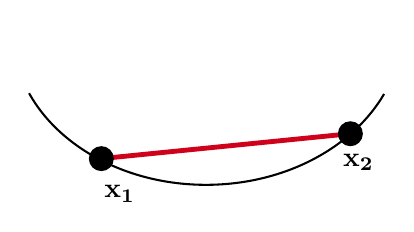
\begin{tikzpicture}[x=0.75pt,y=0.75pt,yscale=-1,xscale=1]
					\draw  [draw opacity=0, line width=1.0pt] (696.23,142.36) .. controls (681.43,167.71) and (649.5,185.54) .. (612.24,186.11) .. controls (573.51,186.7) and (539.97,168.5) .. (525.19,141.99) -- (611.08,111.08) -- cycle ; \draw   (696.23,142.36) .. controls (681.43,167.71) and (649.5,185.54) .. (612.24,186.11) .. controls (573.51,186.7) and (539.97,168.5) .. (525.19,141.99) ;
					\draw [color={rgb, 255:red, 208; green, 2; blue, 27 }  ,draw opacity=1, line width=1.75pt]   (680,161.5) -- (560,173.5) ;
					
					\draw [color={rgb, 255:red, 208; green, 2; blue, 27 }  ,draw opacity=1 ]   (680,161.5) -- (560,173.5) ;
					%Shape: Circle [id:dp3160827101885906] 
					\draw  [fill={rgb, 255:red, 0; green, 0; blue, 0 }  ,fill opacity=1 ] (554.5,173.5) .. controls (554.5,170.46) and (556.96,168) .. (560,168) .. controls (563.04,168) and (565.5,170.46) .. (565.5,173.5) .. controls (565.5,176.54) and (563.04,179) .. (560,179) .. controls (556.96,179) and (554.5,176.54) .. (554.5,173.5) -- cycle ;
					%Shape: Circle [id:dp16415395117171228] 
					\draw  [fill={rgb, 255:red, 0; green, 0; blue, 0 }  ,fill opacity=1 ] (674.5,161.5) .. controls (674.5,158.46) and (676.96,156) .. (680,156) .. controls (683.04,156) and (685.5,158.46) .. (685.5,161.5) .. controls (685.5,164.54) and (683.04,167) .. (680,167) .. controls (676.96,167) and (674.5,164.54) .. (674.5,161.5) -- cycle ;
					
					\draw (560,185) node [anchor=north west][inner sep=0.75pt]   [align=left] {$\mathbf{x_1}$};
					\draw (675,170) node [anchor=north west][inner sep=0.75pt]   [align=left] {$\mathbf{x_2}$};
				\end{tikzpicture}
				
				\captionof{figure}{Convex function}
			\end{minipage}%
			\begin{minipage}{.7\textwidth}
				\centering
				
				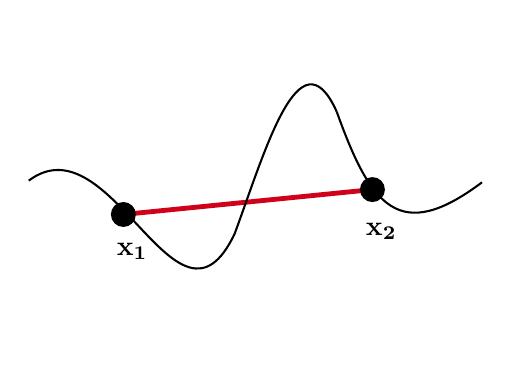
\begin{tikzpicture}[x=0.75pt,y=0.75pt,yscale=-1,xscale=1]
					%uncomment if require: \path (0,300); %set diagram left start at 0, and has height of 300
					
					%Straight Lines [id:da6875192047258083] 
					\draw [color={rgb, 255:red, 208; green, 2; blue, 27 }  ,draw opacity=1, line width=1.75pt]   (564.6,165.5) -- (444.6,177.5) ;
					%Shape: Circle [id:dp14324656781298462] 
					\draw  [fill={rgb, 255:red, 0; green, 0; blue, 0 }  ,fill opacity=1 ] (439.1,177.5) .. controls (439.1,174.46) and (441.56,172) .. (444.6,172) .. controls (447.64,172) and (450.1,174.46) .. (450.1,177.5) .. controls (450.1,180.54) and (447.64,183) .. (444.6,183) .. controls (441.56,183) and (439.1,180.54) .. (439.1,177.5) -- cycle ;
					%Shape: Circle [id:dp2582069443071713] 
					\draw  [fill={rgb, 255:red, 0; green, 0; blue, 0 }  ,fill opacity=1 ] (559.1,165.5) .. controls (559.1,162.46) and (561.56,160) .. (564.6,160) .. controls (567.64,160) and (570.1,162.46) .. (570.1,165.5) .. controls (570.1,168.54) and (567.64,171) .. (564.6,171) .. controls (561.56,171) and (559.1,168.54) .. (559.1,165.5) -- cycle ;
					%Curve Lines [id:da47039197462224447] 
					\draw    (498.2,186.8) .. controls (512.6,148) and (529.4,88) .. (547.4,128) ;
					%Curve Lines [id:da13389450894014865] 
					\draw    (399,161.2) .. controls (439,131.2) and (470.6,244.8) .. (498.2,186.8) ;
					%Curve Lines [id:da2313253314744761] 
					\draw    (547.4,128) .. controls (563.8,173.6) and (577.4,192) .. (617.4,162) ;
					
					\draw (440,190) node [anchor=north west][inner sep=0.75pt]   [align=left] {$\mathbf{x_1}$};
					\draw (560,180) node [anchor=north west][inner sep=0.75pt]   [align=left] {$\mathbf{x_2}$};
				\end{tikzpicture}
				
				\captionof{figure}{Non-convex function}
			\end{minipage}
		\end{figure}
		
		
	\end{flushleft}
\end{frame}



\begin{frame}{Convex functions - examples}
	% \framesubtitle{Part 3}
	\begin{flushleft}
		
		Here are some single-variable convex functions: 
		
		\begin{itemize}
			\item $f(x) = 1$
			\item $f(x) = x$, $f(x) = x + 1$, $f(x) = 6x + 3$
			\item $f(x) = x^2$, $f(x) = (x - 5)^2$, $f(x) = (x + 1)^2 - 10$
			\item $f(x) = x^3$, if $x > 0$
		\end{itemize}
		
		\bigskip
		
		Here are some multi-variable convex functions: 
		
		\begin{itemize}
			\item $f(\mathbf{x}) = \mathbf{A}\mathbf{x} + \mathbf{b}$
			\item $f(\mathbf{x}) = \mathbf{x}^\top \mathbf{H}\mathbf{x}$, $\mathbf{H} \succ 0$ 
		\end{itemize}
		
	\end{flushleft}
\end{frame}



\begin{frame}{Convex programming}
	% \framesubtitle{Part 3}
	\begin{flushleft}
		
		\begin{block}{Definition 3}
			If the domain of the optimization problem is convex and the cost function is convex, it is called a \emph{convex optimization problem}.
		\end{block}
		
		\bigskip
		
		Additionally, we will always assume that the domain of the convex optimization problem contains its boundary. Also, without the loss of generality, we will consider only minimization problems.
		
		\bigskip
		
		There are a few important properties of convex optimization problems (with our additional assumption):
		
		\begin{itemize}
			\item If the domain is non-empty, there is a solution.
			\item The problem has no local minima. We can find a path from any point to the solution, along which the cost function will not increase.
		\end{itemize}
		
	\end{flushleft}
\end{frame}




\myqrframe

\end{document}
